\section{Introduzione teorica e descrizione dell'apparato sperimentale}
Le misure sono state raccolte con due configurazioni ottiche differenti. 
\begin{figure}[h!]
    \centering
    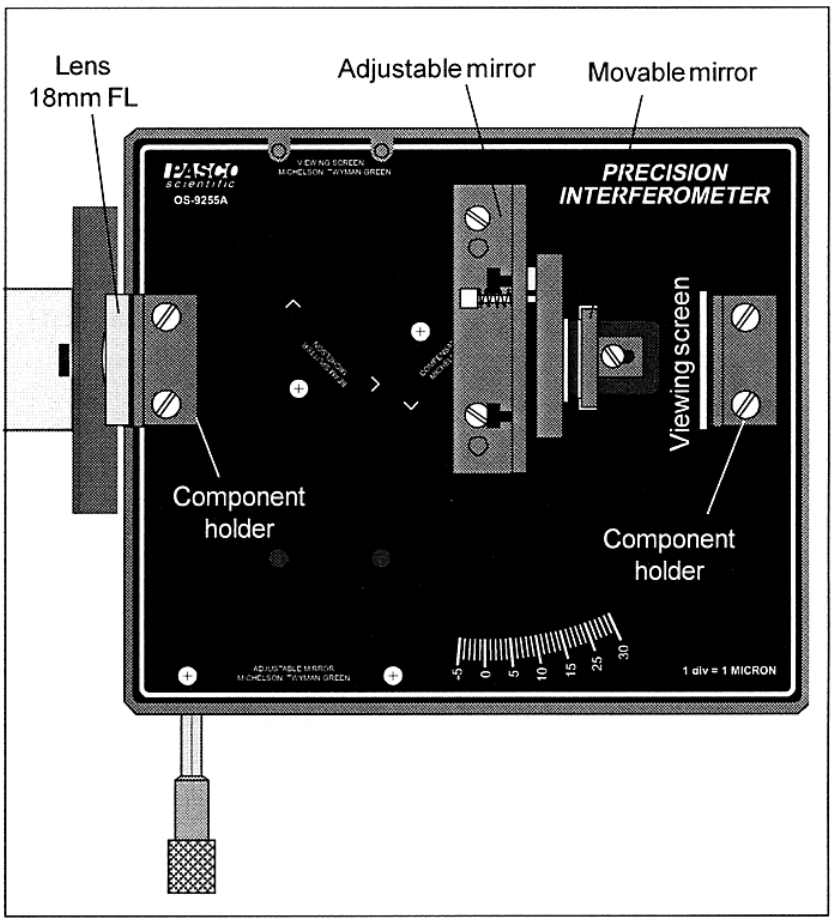
\includegraphics[scale=.45]{immagini/faby pero.png}
    \caption{Configurazione di Fabry-Perot}
    \label{fabi pero}
\end{figure}
In primis abbiamo operato con il sistema ottico di \textit{Fabry-Perot}. L'apparato rappresentato in Figura \ref{fabi pero} è costituito da una base con le indicazioni per posizionare correttamente le lenti necessarie durante l'esperienza; una lente convergente da $18\,mm$, specchi (uno mobile e uno fisso) e un nonio, necessario per regolare in maniera precisa la distanza tra lo specchio fisso e quello mobile. Esterno alla base abbiamo posizionato il banco ottico con la sorgente laser (rosso), allineandolo agli specchi e alle lenti.

In questa configurazione la luce proveniente dalla sorgente laser è posizionata in modo tale che il fascio incida perpendicolarmente allo specchio nel centro e ritorni coincidente con la sorgente. Il raggio è soggetto al fenomeno dell'interferenza, reso visibile grazie alla presenza della lente che lo fa divergere.

Un'interferenza si verifica quando in un punto dello spazio due o più onde si sommano in modo coerente, caratterizzando l'onda risultante con massimi e minimi di ampiezza, e quindi di intensità. Questi ultimi non necessariamente coincidono con le somme dei massimi e minimi delle onde originarie.

Nella nostra esperienza l'interferenza si manifesta tramite dei cerchi concentrici luminosi proiettati su una superficie posta ad almeno un metro di distanza.

Nella configurazione di \textit{Fabry-Perot} si crea una figura di interferenza data da una doppia riflessione del raggio tra i due specchi, che permette di ottenere un effetto simile a quello che si avrebbe in presenza di più sorgenti luminose.

Nella cavità il raggio resta in parte indeviato e viene in parte riflesso raggiungendo lo schermo con uno sfasamento $\delta_r$ che dipende dalla differenza di cammino ottico; cambiando la distanza tra i due specchi, infatti, si osserva lo scorrimento delle frange di interferenza. 

La differenza di fase $\delta$ non tiene conto solo del differente cammino ottico ma anche di uno sfasamento, nel nostro caso considerato trascurabile. Si presenta un'interferenza costruttiva quando la differenza di fase è data da
$$
\delta=2N\pi 
$$
ovvero quando si sommano in fase le ampiezze delle due onde. Si può, quindi, descrivere la figura di interferenza attraverso la relazione
\begin{equation}
    \delta_r \dfrac{\lambda}{2\pi}+2\cdot\cos\theta=N\lambda
\end{equation}
dove $\lambda$ è la lunghezza d'onda del laser, il quale nel nostro caso è a He-Ne e ha $\lambda=632.8\,nm$, mentre $\theta$ è l'angolo ottenuto dalla relazione 
$$
\cos\theta=\dfrac{r}{D}
$$
dove $r$ è la distanza rispetto al centro della figura di interferenza del massimo che si utilizza come riferimento e $D$ è la distanza tra la sorgente dell'interferenza e lo schermo rilevatore.
\begin{figure}[h!]
    \centering
    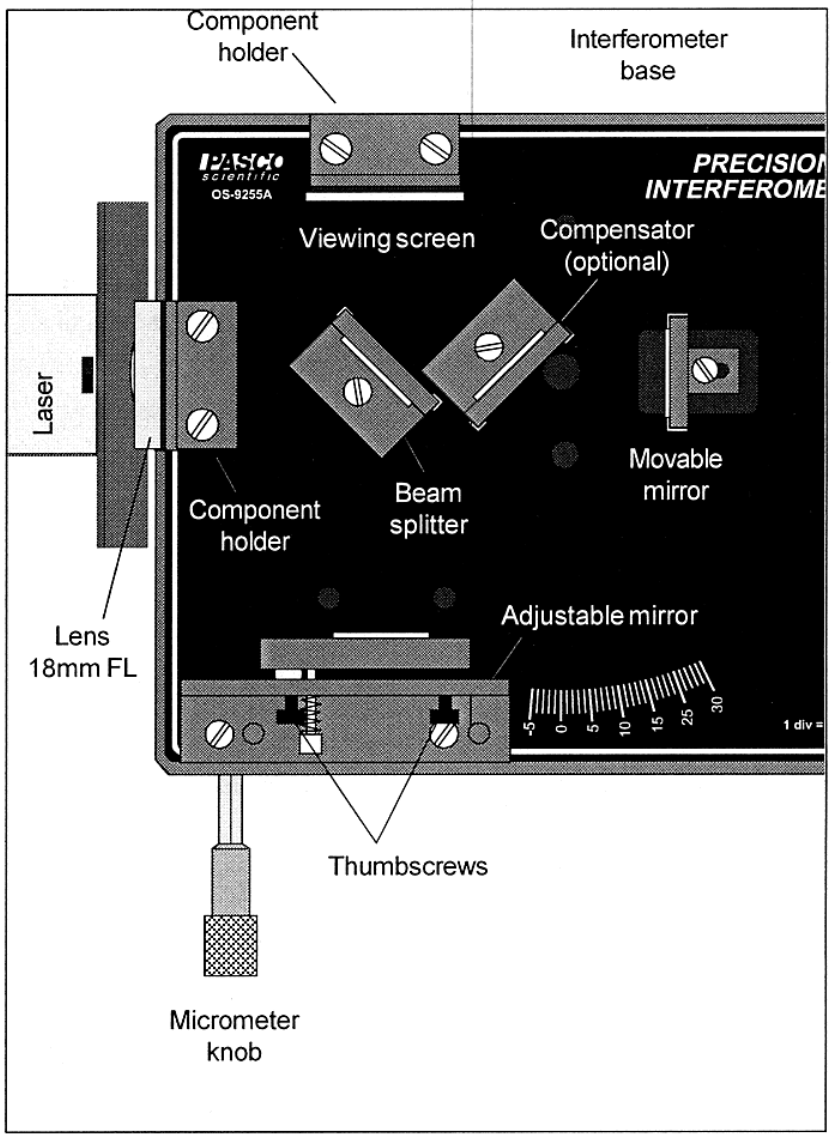
\includegraphics[scale=.37]{immagini/michaelson.png}
    \caption{Configurazione di Michelson}
    \label{michelino}
\end{figure}
Lo scopo di questa parte di esperienza è, perciò, quello di verificare la legge e, dopo aver calibrato il nonio, determinare la lunghezza d'onda di un secondo laser di $\lambda$ ignota.
\\

In secondo luogo abbiamo operato con la configurazione di \textit{Michelson}. In maniera analoga a quella illustrata precedentemente abbiamo allineato il banco ottico, modificando però la posizione degli specchi. Abbiamo utilizzato questa configurazione per determinare l'indice di rifrazione dell'aria e quello del vetro. Nel primo caso ci siamo serviti di una pompa in grado di creare una differenza di pressione all'interno della cella; nel secondo caso abbiamo, invece, fatto uso di uno strumento che ci permettesse di ruotare una lastra di vetro, così da determinarne l'indice di rifrazione alla variazione dell'angolo di incidenza.

Nel primo caso la relazione che descrive la legge è
\begin{equation}
   \eta_{\text {aria }}=\dfrac{\Delta N\,\lambda}{2d(P_i-P_f)}
   \label{aria}
\end{equation}
mentre nel secondo caso, invece, è
\begin{equation}
\eta_{\text {vetro }}=\frac{(2 d-\Delta N \lambda)(1-\cos \theta)}{2 d \cdot(1-\cos \theta)-\Delta N \lambda}
\label{eq 3}
\end{equation}
